\documentclass[a4paper, 12pt, spanish]{article}

\usepackage[paper=a4paper, left=1.5cm, right=1.5cm, bottom=1.5cm, top=3.5cm]{geometry}
\usepackage[spanish, es-noshorthands]{babel}
\usepackage[utf8x]{inputenc}
\usepackage[none]{hyphenat}
\usepackage[colorlinks,citecolor=black,filecolor=black,linkcolor=black,    urlcolor=black]{hyperref}

% Simbolos matemáticos
\usepackage{amsthm}
\usepackage{amsmath}
\usepackage{amsfonts}
\usepackage{amssymb}
\usepackage{listings}

% Descoración y gráficos
\usepackage{caratulaV}
\usepackage{graphicx}
\usepackage{longtable}
\usepackage{fancyhdr}
\usepackage{lastpage}
\usepackage{caption}
\usepackage{subcaption}
\usepackage{multirow}
\usepackage{alltt}
\usepackage{tikz}
\usepackage{color}
\usepackage{verbatim}
\usepackage{framed}
\newenvironment{reglas}
{   \begin{tabular}{lcl} }
{ \end{tabular}\\ }
\newcommand*{\thead}[1]{%
\multicolumn{1}{c}{\bfseries\begin{tabular}{@{}c@{}}#1\end{tabular}}}
\newcommand*{\tcell}[1]{%
\multicolumn{1}{c}{\begin{tabular}{@{}c@{}}#1\end{tabular}}}
\newcommand{\regla}[2]{#1 & $\to$ & #2 \\ }%
\newcommand{\aregla}[1]{\ &  $|$  & #1 \\ }%
\newcommand{\newToken}[2]{\newcommand{#1}{\textbf{#2} }}
% Bibliografía
\usepackage{natbib}

% Del enunciado
\usepackage{a4wide}
\usepackage{amsmath}
\usepackage{amsfonts}
\usepackage{graphicx}
%\usepackage[ruled,vlined]{algorithm2e}

% Del enunciado
\usepackage{pdfpages}

\newcommand{\kknn}{k}
\newcommand{\kpca}{\alpha}
\newcommand{\kkfold}{K}

% Acomodo fancyhdr.
\pagestyle{fancy}
\thispagestyle{fancy}
\addtolength{\headheight}{1pt}
\lhead{Teoría de Lenguajes}
\rhead{$1^{\mathrm{er}}$ cuatrimestre de 2016}
\cfoot{\thepage /\pageref*{LastPage}}
\renewcommand{\footrulewidth}{0.4pt}

\sloppy

\parskip=5pt % 10pt es el tama de fuente

% Pongo en 0 la distancia extra entre itemes.
\let\olditemize\itemize
\def\itemize{\olditemize\itemsep=0pt}


%\materia{Métodos Númericos}
%\grupo{Conformación del grupo}
%\tituloCaratula{Trabajo Práctico N$^\circ$1\\ \vspace{0.5cm} ``No creo que a él le gustará eso''}


\usepackage{tikz}
%\usepackage{tikz-qtree}


\usetikzlibrary{arrows,backgrounds,calc}

\pgfdeclarelayer{background}
\pgfsetlayers{background,main}

\newcommand{\real}{\mathbb{R}}
\newcommand{\nat}{\mathbb{N}}

\newcommand{\revJ}[1]{{\color{red} #1}}

\newcommand{\convexpath}[2]{
[
    create hullnodes/.code={
        \global\edef\namelist{#1}
        \foreach [count=\counter] \nodename in \namelist {
            \global\edef\numberofnodes{\counter}
            \node at (\nodename) [draw=none,name=hullnode\counter] {};
        }
        \node at (hullnode\numberofnodes) [name=hullnode0,draw=none] {};
        \pgfmathtruncatemacro\lastnumber{\numberofnodes+1}
        \node at (hullnode1) [name=hullnode\lastnumber,draw=none] {};
    },
    create hullnodes
]
($(hullnode1)!#2!-90:(hullnode0)$)
\foreach [
    evaluate=\currentnode as \previousnode using \currentnode-1,
    evaluate=\currentnode as \nextnode using \currentnode+1
    ] \currentnode in {1,...,\numberofnodes} {
-- ($(hullnode\currentnode)!#2!-90:(hullnode\previousnode)$)
  let \p1 = ($(hullnode\currentnode)!#2!-90:(hullnode\previousnode) - (hullnode\currentnode)$),
    \n1 = {atan2(\x1,\y1)},
    \p2 = ($(hullnode\currentnode)!#2!90:(hullnode\nextnode) - (hullnode\currentnode)$),
    \n2 = {atan2(\x2,\y2)},
    \n{delta} = {-Mod(\n1-\n2,360)}
  in
    {arc [start angle=\n1, delta angle=\n{delta}, radius=#2]}
}
-- cycle
}

\newcommand{\todo}[1]{
\textbf{\color{red}{\underline{Nota:} #1}}
}

\newcommand\param[3]{\ensuremath{\mathbf{\textbf{#1}}\,#2\!:} \texttt{#3}}


\newcommand{\degree}{\ensuremath{^\circ}}

\begin{document}
%\setcounter{tocdepth}{2}
\renewcommand{\tablename}{Tabla}


\thispagestyle{empty}
\materia{Redes Neuronales}
\submateria{Primer Cuatrimestre de 2017}
\titulo{Trabajo Práctico}
\subtitulo{\emph{Redes feedforward multicapa}}
\integrante{Juan Cruz Sosa}{733/12}{nirvguy@gmail.com}
\integrante{Martín Caravario}{470/12}{martin.caravario@gmail.com}
\maketitle
\newpage
%\begin{titlepage}

%\maketitle

%\end{titlepage}
\setcounter{page}{1}
\newpage
\section{Introducción}


\section{Modo de uso y requerimientos}
Para correr este programa es necesario contar con Python 3 instalado junto a los paquetes Numpy y Pandas. Ambos paquetes pueden descargarse a traves
de la herramienta pip de python mediante el comando
\begin{verbatim}
  sudo pip3 install pandas
  sudo pip3 install numpy
\end{verbatim}
En caso de no tener instalada la herramienta pip, puede hacer con el comando
\begin{verbatim}
  sudo apt-get install python3-pip
\end{verbatim}

Para utilizar el programa debe posicionarse en la carpeta correspondiente al ejercicio que se desea correr. Luego se debe ejecutar el siguiente comando
\begin{verbatim}
  python3 ej unidades af -t tm -n eta -e epochs -a a -b b --alpha alpha
          --batch_size bs --training-prop tp --random-funct rf --normalize-input
          --no-normalize-input --normalize-output  --no_normalize-output
          --test --train --db
\end{verbatim}

en donde:
\begin{itemize}
  \item \textbf{ej}: es el ejericio que se va a correr, sus valores pueden ser {ej1.py, ej2.py}
  \item \textbf{unidades}: es la cantidad de unidades por capa, por ejemplo 10-20-1
  \item \textbf{af}: son las funciones de activacion que se utilizaran para cada capa intermedia de la red. Sus valores pueden ser: s (funcion signo), t (tangente hiperbolica),
                    l (sigmoidea), r (ReLu), i (funcion identidad). Las funciones deben ir separadas por un guion, por ejemplo l-t-s.
  \item \textbf{tm}: es el modo de entrenamiento, sus valores pueden ser {stochastic, online, batch, mini\_batch}. En caso de ser mini\_batch la opcion seleccionada se debera
            proveer el tamaño del batch a utilizar mediante la opcion --batch\_size bs, en donde bs será el tamaño en cuestion.
  \item \textbf{n}: es el coeficiente de entrenamiento $\eta$ que se utilizará en el entrenamiento
  \item \textbf{epochs}: es la cantidad de epocas que se utilizaran para el entrenamiento
  \item \textbf{a}: es el coeficiente a correspondiente al correspondiente parametro adaptativo de entrenamiento
  \item \textbf{b}: es el coeficiente b correspondiente al correspondiente parametro adaptativo de entrenamiento
  \item \textbf{alpha}: es un parametro opcional que se utiliza en caso de querer utilizar la optimizacion de momentum para el algoritmo de BackPropagation. Corresponde al $\alpha$
                correspondiente.
  \item \textbf{tp}: es un parametro opcional que representa la proporcion correspondiente del set de datos que se utilizara como datos de entrenamiento,
            mientras que el resto se utilzara como datos de validacion. El valor de tp provisto debe ser 0 < tp < 1.
  \item \textbf{rf}: es un parametro opcional que selecciona el valor de la funcion random que se utilizara para la inicializacion de los pesos en la matriz de pesos de la red.
            Sus valores pueden ser {normal, uniform}
  \item \textbf{--test}: es un parametro opcional que indica que se utilizara la mejor red entrenada por el grupo para testear sobre el set de datos que se pasan en el parametro
                        --db. Es decir que evaluara el set de datos con la mejor red entrenada.
  \item \textbf{--train}: es un parametro opcional que especifica que se entrenara la red pasada como parametro y se utilizara el set de datos pasados en el parametro --db
                        como conjunto de datos de entrenamiento.
  \item \textbf{--db}: es un parametro opcional que especifica la base de datos que se utilizara ya sea para entrenar una nueva red si esta activada la opcion --train, o
                        para testear la mejor red obtenida en caso de que este el parametro --test.
  \item \textbf{--no-normalize-input}: es un parametro opcional que especifica que no se normalice la entrada
  \item \textbf{--normalize-input}: es un parametro opcional que especifica que se normalice la entrada
  \item \textbf{--normalize-output}: es un parametro opcional que especifica que se normalice la salida
  \item \textbf{--no-normalize-output}: es un parametro opcional que especifica que no se normalice la salida
\end{itemize}

En caso de querer consultar el modo de uso manualmente puede hacerse mediante el comando
\begin{verbatim}
    sudo python3 ej -h
\end{verbatim}
en donde ej puede ser {ej1.py, ej2.py}
%
% -t {stochastic,online,batch,mini_batch}, --training-mode {stochastic,online,batch,mini_batch}
%                        Modo de entrenamiento
%  -n ETA, --eta ETA
%  -e EPOCHS, --epochs EPOCHS
%  --alpha ALPHA
%  -a A, --a A
%  -b B, --b B
%  --batch_size BATCH_SIZE
%  --training-prop TRAINING_PROP
%  --normalize-input
%  --no-normalize-input
%  --normalize-output
%  --no_normalize-output
%  --random-funct {normal,uniform}

\newpage

\tableofcontents
\newpage
\section{Ejercicio 1}

\subsection{Introducción}
Este ejercicio consiste en entrenar una red neuronal que, dados los resultados de un examen específico que es utilizado en el diagnóstico del
cáncer de mamas, sepa clasificar ese conjunto dentro de dos categorias posibles: B y M. Para el este ejercicio B significará que el tumor diagnosticado
es benigno y M será maligno.

\subsection{Experimentación}
Al ser un ejercicio de clasificacion la red neuronal deberá devolver un valor para cada clase, por lo que la ultima función de activacion necesariamente
deberá devolver unicamente dos valores posibles. En este caso se utilizó la función signo bipolar, la cual devolvera -1 en caso de la muestra pertenecer
a la clase M (Maligno) y 1 en caso contrario la clase B (Benigno).

Tambien se decidió utilizar el 60\% de los datos como datos de entrenamiento y el 40\% restante como datos de validacion. Esta eleccion se debe a que
queremos poder extraer una mayor cantidad de informacion del entramiento, antes de pasar a clasificar nuevos datos.

\subsubsection{Experimento 1}
Este experimento consistió en comparar distintas arquitecturas de redes neuronales variando la cantidad de capas ocultas y de neuronas por capa.
Para este experimento se decidió fijar el coeficiente de aprendizaje $\eta$ en 0.03, la cantidad de epocas sobre las que se entrena la red en 1000 y el
método de entrenamiento estocástico. Con respecto a las funciones de activación se utilizaron sigmoideas para las capas intermedias y la función signo
para la capa final.

Las redes que se utilizaron fueron las siguientes:
\begin{enumerate}
  \item 10 - 1 (Perceptron simple): Esta red se planteó para ver si el problema era linealmente separable y podia ser aprendido por un perceptron
                                      simple.
  \item 10 - 20 - 1: Esta red se planteo para extraer una cantidad de features mayor a la cantidad de datos de entrada del problema y asi poder sintetizar
                      estos en la neurona de salida.
  \item 10 - 5 - 5 - 8 - 1: Esta red se planteo para analizar el comportamiento de la red al agregarle mas etapas de procesamiento anidadas.
\end{enumerate}

Los resultados que se obtuvieron fueron los siguientes:
\begin{figure}[h!]
  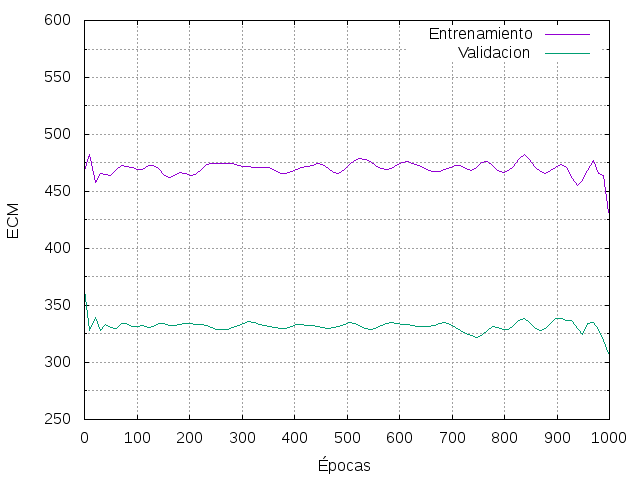
\includegraphics[width=125mm]{imagenes/ej1/ex_1-1_red_11-1_errors.png}
  \caption{Red 1}
\end{figure}

\begin{figure}[h!]
  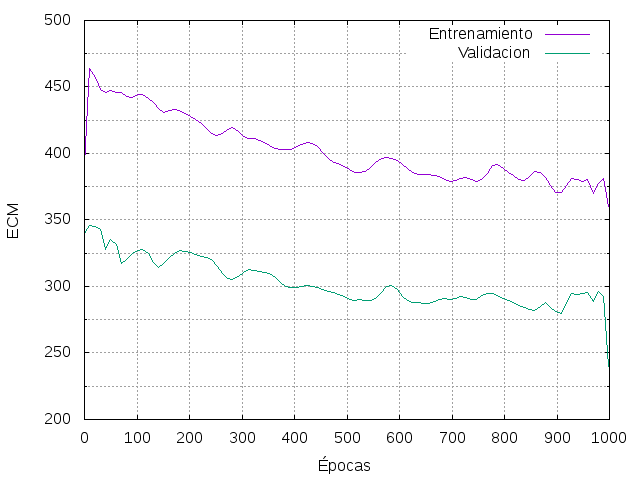
\includegraphics[width=125mm]{imagenes/ej1/ex_1-1_red_11-6-6-9-1_errors.png}
  \caption{Red 2}
\end{figure}

\begin{figure}[h!]
  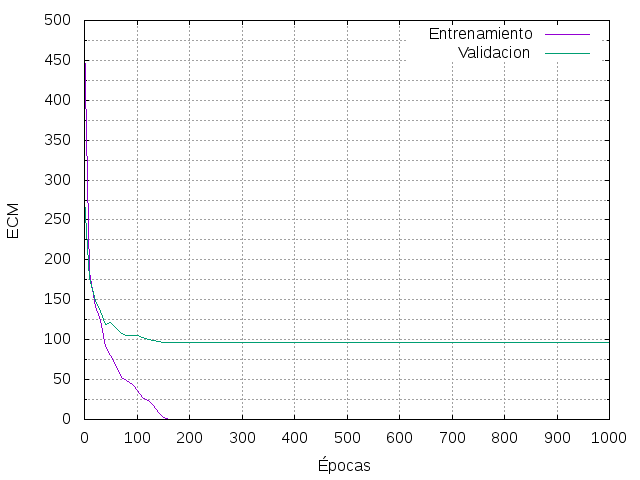
\includegraphics[width=125mm]{imagenes/ej1/ex_1-1_red_11-21-1_errors.png}
  \caption{Red 3}
\end{figure}


 Tal como se observa en los resultados de la Red 1, la cual es un perceptrón simple, el error cuadratico medio (ECM) no es notorio un decrecimiento (aun mas una oscilacion
 muy variada) de esta a medida que aumentan las epocas.
 Esto tambien se evidencia en la tabla de aciertos en la cual logra un 62.60\% de aciertos sobre los datos de entrenamiento y un 61.58\% sobre datos de validación,
 lo cual es bastante bajo siendo 1000 la cantidad de epocas con las que se entrena. Ademas analizando las columnas de falsos positivos y falsos negativos no se observó
 predominancia de un tipo de error sobre el otro, es decir que casi la mitad de las veces se observan falsos negativos, lo cual no es deseable para el dominio de este problema.
 Con toda la evidencia provista por los graficos se estimó que el problema a resolver no es linealmente separable pues no es posible
 aprenderlo con un perceptrón simple, por lo tanto esta red se descartó para futuros experimentos ya que sus resultados no fueron relevantes.

 Con respecto a la Red 2, se observa que el ECM decrece casi linealmente tanto en validacion como en entrenamiento, comenzando en 340 sobre validacion y
 logrando un valor minimo de 96. En la tabla de aciertos se observa un 99.59\% de aciertos sobre entrenamiento y un 89.02\% sobre validacion. Tambien se observa
 que el ritmo de aprendizaje es inferior con respecto a la Red 3 pero es superior al de la Red 1, sin embargo, dados los resultados obtenidos se consideró
 que puede ser notablemente mejorada con una optimizacion del algoritmo de BackPropagation, por lo que se decidió continuar experimentado sobre ella.

 Finalmente, la red 3 es la que mejor aprende de los datos de entrenamiento llegando al valor minimo absoluto de 0 en ECM sobre los datos de entrenamiento y un valor minimo
 de 96 en ECM sobre datos de validación. Tambien se observa que la funcion del ECM decrece rapidamente por lo que se concluye que este perceptron multicapa
 logra aprender en solo 150 epocas todo el set de entrenamiento. Esto trae como desventaja el hecho de que no se podrá disminuir mucho mas el ECM puesto que el set
 de entrenamiento fue completamente aprendido y luego de esto el ECM del set de validacion se mantendrá constante.
 A pesar de esto, en la tabla de aciertos se observó un alto
 porcentaje de aciertos, 100\% y 89.63\% para entrenamiento y validacion respectivamente por lo que se decidió seguir utilizando esta red para futuros experimentos
 con el objetivo de mejorar el porcentaje de aciertos sobre validacion al hacer mejoras al algoritmo de BackPropagation.

\subsubsection{Experimento 2}
Para este experimento se decidió variar el coeficiente de aprendizaje $\eta$ e introducir la optimizacion del \textit{momentum} al algoritmo de BackPropagation,
variando su respectivo parametro $\alpha$. Esto permite darle una aceleracion o decaiminento al nivel de aprendizaje en base al valor del parametro.
Las redes utilizadas fueron las redes 2 y 3 del Experimento 1, con 1000 epocas y continuando con el modo entrenamiento estocastico.
El valor de $\eta$ lo variamos con los siguientes valores: 0.03 y 0.07, mientras que el valor de $\alpha$ se varió con los valores: 0.1 y 0.3,
con lo cual se obtuvieron 4 combinaciones posibles para cada red. Estos valores se elegieron dentro de lo razonable (valores de $\eta$ mayores a 0.1
representan un cambio brusco en el aprdendizaje) para representar las posibles combinaciones de $\eta$ chico/grande junto a un $\alpha$ chico/grande y
 asi poder analizar diversos comportamientos de la red.

 Los resultados obtenidos se presentan a continuacion:

\begin{figure}[h!]
  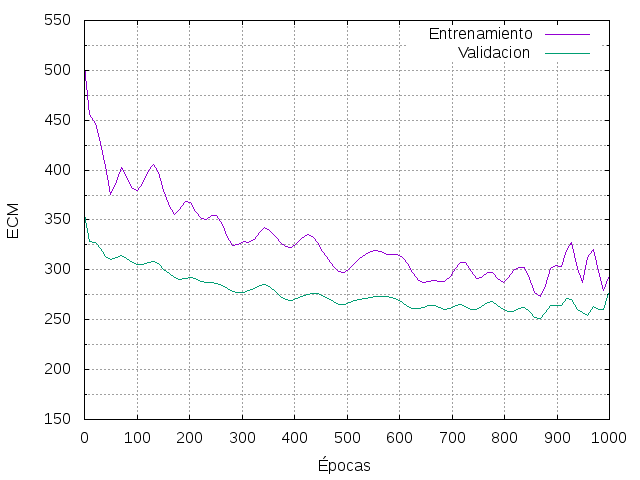
\includegraphics[width=125mm]{imagenes/ej1/ex_2-1_red_11-6-6-9-1_errors.png}
  \caption{Red 3 con parametros $\eta = 0.07$ y $  \alpha = 0.1$}
\end{figure}

\begin{figure}[h!]
  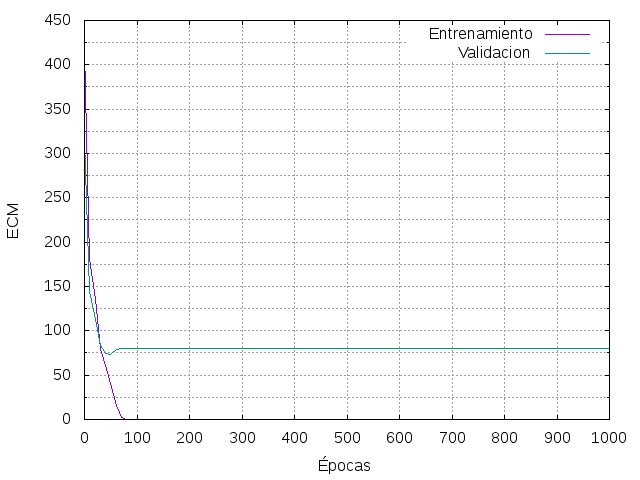
\includegraphics[width=125mm]{imagenes/ej1/ex_2-1_red_11-21-1_errors.png}
  \caption{Red 2 con parametros $\eta = 0.07$ y $  \alpha = 0.1$}
\end{figure}

\begin{figure}[h!]
  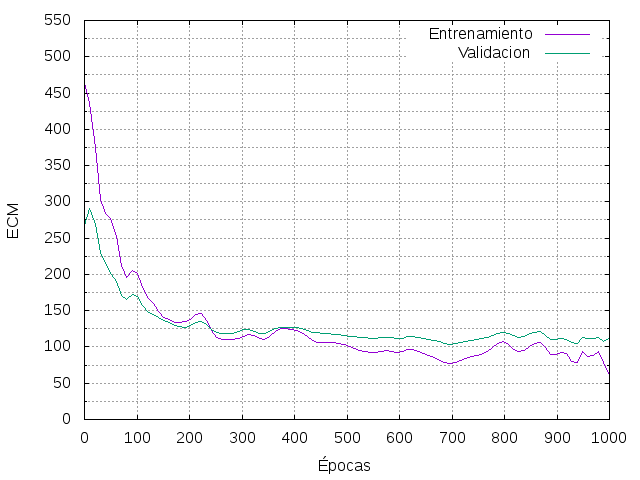
\includegraphics[width=125mm]{imagenes/ej1/ex_2-2_red_11-6-6-9-1_errors.png}
  \caption{Red 3 con parametros $\eta = 0.03$ y $\alpha = 0.1$}
\end{figure}

\begin{figure}[h!]
  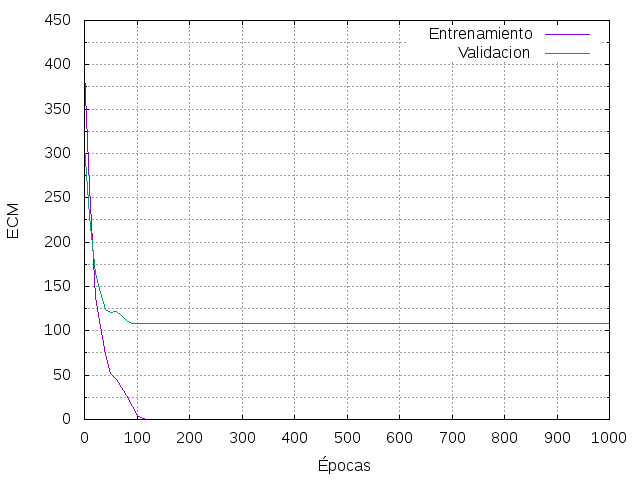
\includegraphics[width=125mm]{imagenes/ej1/ex_2-2_red_11-21-1_errors.png}
  \caption{Red 2 con parametros $\eta = 0.03$ y $  \alpha = 0.1$}
\end{figure}

\begin{figure}[h!]
  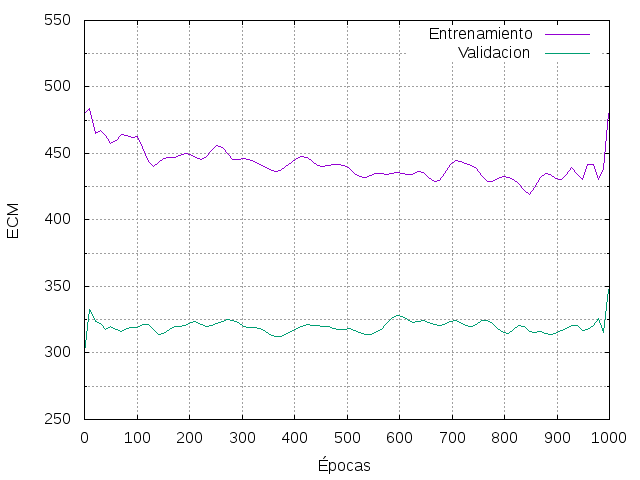
\includegraphics[width=125mm]{imagenes/ej1/ex_2-3_red_11-6-6-9-1_errors.png}
  \caption{Red 3 con parametros $\eta = 0.03 $ y $ \alpha = 0.3$}
\end{figure}

\begin{figure}[h!]
  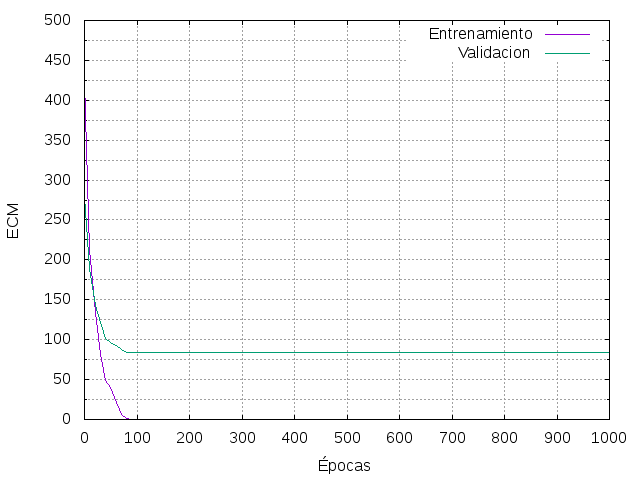
\includegraphics[width=125mm]{imagenes/ej1/ex_2-3_red_11-21-1_errors.png}
  \caption{Red 2 con parametros $\eta = 0.03 $ y $ \alpha = 0.3$}
\end{figure}

\begin{figure}[h!]
  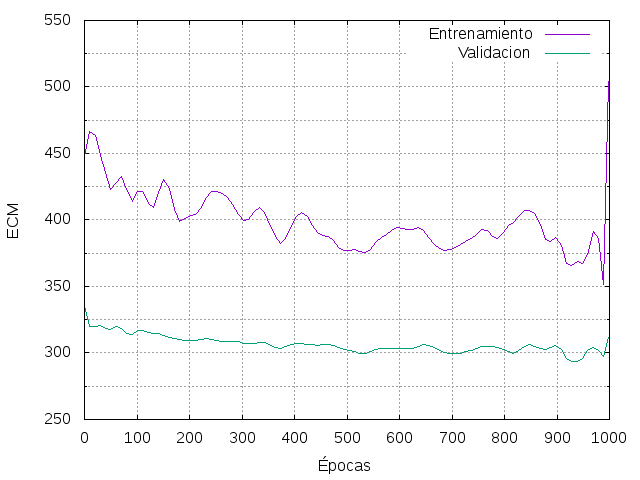
\includegraphics[width=125mm]{imagenes/ej1/ex_2-4_red_11-6-6-9-1_errors.png}
  \caption{Red 3 con parametros $\eta = 0.07 $ y $ \alpha = 0.3$}
\end{figure}

\begin{figure}[h!]
  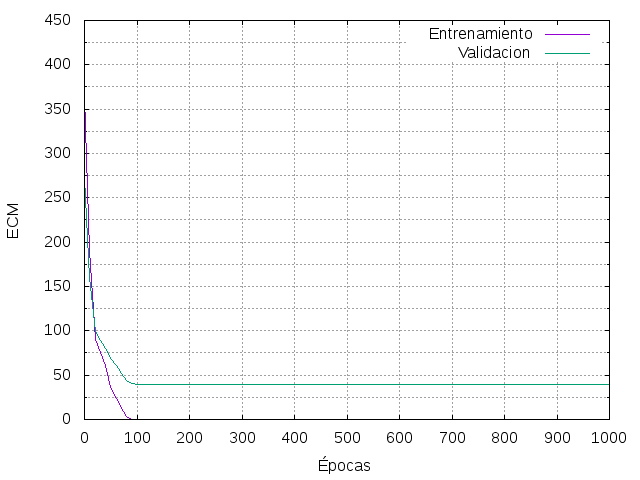
\includegraphics[width=125mm]{imagenes/ej1/ex_2-4_red_11-21-1_errors.png}
  \caption{Red 2 con parametros $\eta = 0.07 $ y $ \alpha = 0.3$}
\end{figure}

Se observa que la mejor combinacion de parametros para la Red 2, es aquella en la cual $\eta = 0.07$ y $\alpha = 0.3$, pues presenta los valores
mas bajos de ECM en validacion, alcanzando valores por debajo de 50. Con respecto a la cantidad de aciertos para estos parametros se obtiene un
93.90\% en datos de validacion y a su vez se obtiene la misma cantidad de falsos positivos como de falsos negativos en caso de fallos.
 Esto mejora ampliamente los resultados obtenidos en el experimento 1 y contradice el hecho de que el ECM no podia disminuir mas debido a la veloz
 convergencia.

Con respecto a la Red 3, la mejor combinacion de parametros fue $\eta = 0.03$ y $\alpha = 0.1$, en la cual se observan valores de ECM por debajo de 150
en validacion. Tambien se observa una mejora en la cantidad de aciertos obteniendo un valor de 88.41\%, esta mejora de un 20\% con respecto al experimento
anterior, validan la hipotesis de que esta red podia ser aun mas optimizada para poder competir con la eficiencia de la Red 2.


A raíz de estos experimentos se concluyó que para la Red 2 una mayor influencia de los pesos de las epocas anteriores genera una mejora en la performance
de esta red. En cambio, la Red 3 al agregar una minima proporcion de los pesos de las epocas anteriores genera una importante mejora en la eficiencia
de la red.
Finalmente para el resto de la experimentacion se decidio descartar la Red 2 debido a que obtuvo una mejora de solo un 3\% en la cantidad de aciertos,
mientras que la Red 3 obtuvo un 20\%.

\subsubsection{Experimento 3}
Para este experimento se decidió experimentar con parametros adaptativos y sus respectivos coeficientes $a$ y $b$. Se utilizó la Red 3 definida
previamente, fijando la cantidad de epocas en 1000, continuando aun con el modo de entrenamiento estocástico, $\eta = 0.03$ y $\alpha = 0.1$ ( producto
de los mejores parametros del experimento anterior).
Con respecto a los coeficientes de los parametros adaptativos, se fijo $a = 0.02$ y $b$ se varió con los valores: 0.7 y 0.1. La eleccion del $a$ se debe
a que en caso de disminuir el error se buscó aumentar el $\eta$, pero que la diferencia de salto no sea muy grande o se mantenga chica. Los valores de
 $b$ representan la disminucion de un porcentaje del valor del $\eta$ anterior, produciendo que los saltos sean mas finos, y es por esto que se decidió
 tomar un valor representantivo grande(0.7) y otro chico(0.1).

Los resultados obtenidos fueron los siguientes:
\begin{figure}[h!]
  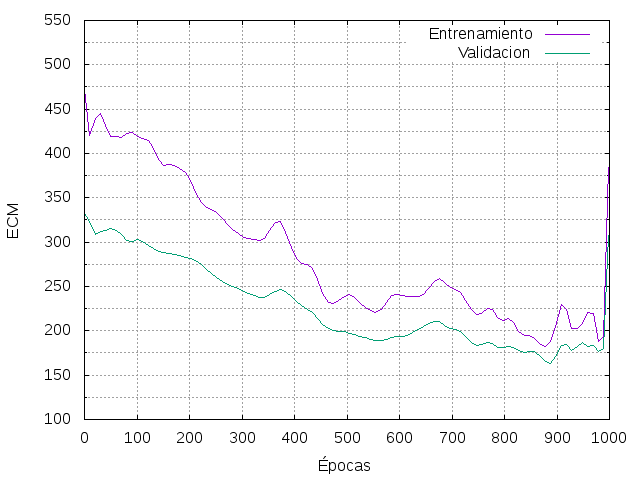
\includegraphics[width=125mm]{imagenes/ej1/ex_3-1_red_11-6-6-9-1_errors.png}
  \caption{Red 3 con parametros $a = 0.02 $ y $b= 0.7$}
\end{figure}

\begin{figure}[h!]
  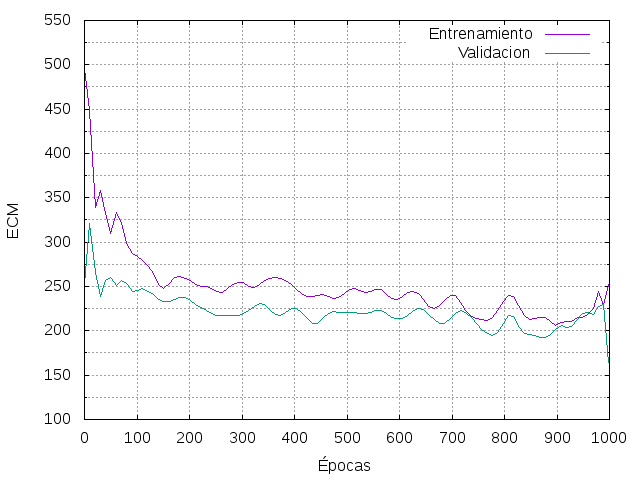
\includegraphics[width=125mm]{imagenes/ej1/ex_3-2_red_11-6-6-9-1_errors.png}
  \caption{Red 2 con parametros $a = 0.02 $ y $b = 0.1$}
\end{figure}

Sobre estos resultados no se observó una mejora con respecto a los obtenidos en el experimento anterior por lo cual estos parametros no serán
tenidos en cuenta para el resto de la experimentacion.

\subsubsection{Experimento 4}
Para este experimento se decidió variar el modo de entrenamiento entre \textit{Batch} y \textit{Mini Batch}. Para este ultimo se tomó como tamaño
de batch los valores 10 y 30. Con respecto a los valores restantes se utilizaron los mismos a la configuracion del Experimento 3.

Los resultados obtenidos fueron los siguientes:

\begin{figure}[h!]
  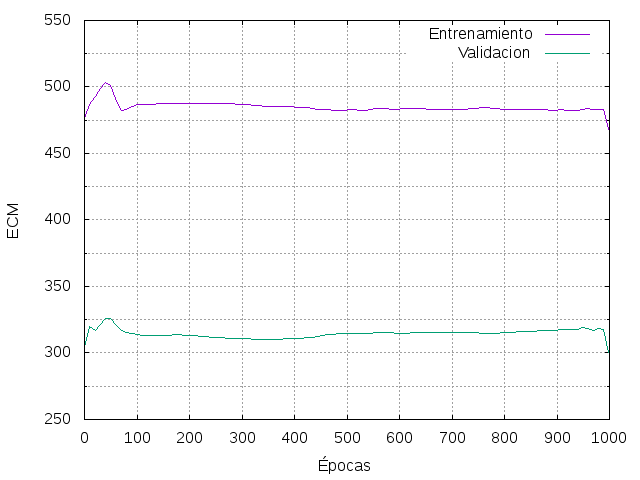
\includegraphics[width=125mm]{imagenes/ej1/ex_4-1_red_11-6-6-9-1_errors.png}
  \caption{Modo de entrenamiento Batch}
\end{figure}

\begin{figure}[h!]
  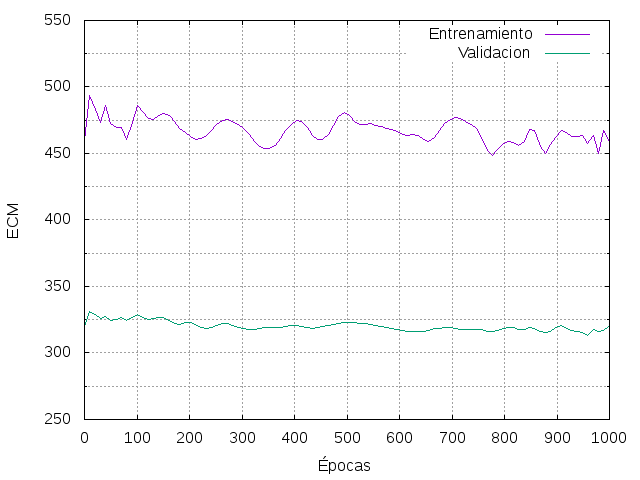
\includegraphics[width=125mm]{imagenes/ej1/ex_4-2_red_11-6-6-9-1_errors.png}
  \caption{Modo de entrenamiento Mini Batch con tamaño de batch 10}
\end{figure}

\begin{figure}[h!]
  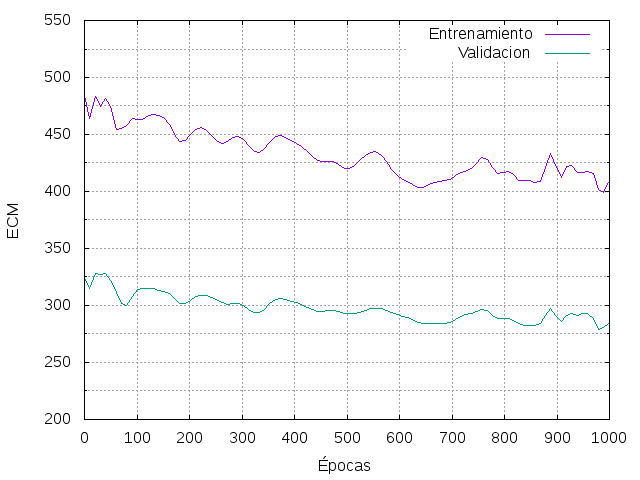
\includegraphics[width=125mm]{imagenes/ej1/ex_4-3_red_11-6-6-9-1_errors.png}
  \caption{Modo de entrenamiento Mini Batch con tamaño de batch 30}
\end{figure}

Se concluyó que esta experimentacion no mejora los resultados obtenidos en experimentos anteriores. Por lo tanto se decidió
mantener el modo de entrenamiento en estocastico, con el cual se obtuvieron los mejores resultados.

\subsection{Tabla de aciertos}
A continuación se presenta la tabla de aciertos con todos los resultados de la experimentación del ejercicio 1.
\begin{table}[h!]
	\begin{tabular}{c|c|c|c|c|c|c}
		Experimento & Red & Parametros & Mejor  de aciertos training & Mejor  de validacion & Mejor  de validacion \\
		1 & 2 & $\eta$ = 0.03, epocas = 1000, Estocastico & 99.59349593495935 (96 epochs) & 89.02439024390245 (88 epochs) &  33.33333333333333 & 66.66666666666666 \\
		1 & 3 & $\eta$ = 0.03, epocas = 1000, Estocastico & 66.66666666666666 (969 epochs) & 64.02439024390245 (916 epochs) &  35.59322033898305 & 64.40677966101694 \\
		1 & 1 & $\eta$ = 0.03, epocas = 1000, Estocastico & 62.601626016260155 (944 epochs) & 61.58536585365854 (394 epochs) &  44.44444444444444 & 55.55555555555556 \\
		2 & 2 & $\eta$ = 0.07, epocas = 1000, Estocastico, $\alpha$ = 0.1 & 98.3739837398374 (55 epochs) & 93.29268292682927 (50 epochs) &  54.54545454545454 & 45.45454545454545 \\
		2 & 3 & $\eta$ = 0.07, epocas = 1000, Estocastico, $\alpha$ = 0.1  & 80.89430894308943 (903 epochs) & 71.34146341463415 (795 epochs) &  80.85106382978722 & 19.148936170212767 \\
		2 & 2 &  $\eta$ = 0.03, epocas = 1000, Estocastico, $\alpha$ = 0.1 & 99.59349593495935 (54 epochs) & 87.8048780487805 (49 epochs) &  40.0 & 60.0 \\
		2 & 3 &  $\eta$ = 0.03, epocas = 1000, Estocastico, $\alpha$ = 0.1 & 96.34146341463415 (934 epochs) & 88.41463414634147 (577 epochs) &  52.63157894736842 & 47.368421052631575 \\
		2 & 2 &  $\eta$ = 0.03, epocas = 1000, Estocastico, $\alpha$ = 0.3 & 99.59349593495935 (58 epochs) & 88.41463414634147 (43 epochs) &  73.68421052631578 & 26.31578947368421 \\
		2 & 3 &  $\eta$ = 0.03, epocas = 1000, Estocastico, $\alpha$ = 0.3 & 64.22764227642277 (766 epochs) & 57.92682926829268 (685 epochs) &  5.797101449275362 & 94.20289855072464 \\
		2 & 3 & $\eta$ = 0.07, epocas = 1000, Estocastico, $\alpha$ = 0.3 & 72.76422764227642 (818 epochs) & 60.97560975609756 (816 epochs) &  59.375 & 40.625 \\
		2 & 2 & $\eta$ = 0.07, epocas = 1000, Estocastico, $\alpha$ = 0.3 & 99.59349593495935 (52 epochs) & 93.90243902439023 (100 epochs) &  50.0 & 50.0 \\
		3 & 3 & $\eta$ = 0.03, epocas = 1000, Estocastico, $\alpha$ = 0.1, $a$ = 0.02, $b$ = 0.7 & 88.6178861788618 (928 epochs) & 79.26829268292683 (880 epochs) &  50.0 & 50.0 \\
		3 & 3 & $\eta$ = 0.03, epocas = 1000, Estocastico, $\alpha$ = 0.1, $a$ = 0.02, $b$ = 0.1 & 84.14634146341463 (968 epochs) & 79.8780487804878 (924 epochs) &  36.36363636363637 & 63.63636363636363 \\
		4 & 3 & $\eta$ = 0.03, epocas = 1000, Batch, $\alpha$ = 0.1 & 52.84552845528455 (61 epochs) & 58.536585365853654 (61 epochs) &  2.941176470588235 & 97.05882352941177 \\
		4 & 3 & $\eta$ = 0.03, epocas = 1000, MiniBatch, batch\_size = 10, $\alpha$ = 0.1 & 65.85365853658537 (863 epochs) & 57.92682926829268 (239 epochs) &  89.85507246376811 & 10.144927536231885 \\
		4 & 3 & $\eta$ = 0.03, epocas = 1000, MiniBatch, batch\_size = 50, $\alpha$ = 0.1 & 71.54471544715447 (986 epochs) & 67.6829268292683 (827 epochs) &  35.84905660377358 & 64.15094339622641 \\
	\end{tabular}
\end{table}



\subsection{Conclusión}

\newpage

\newpage
\section{Mapas Auto-organizados }

\subsection{Introducción}
Este ejercicio consistio en crear un modelo de mapeo de caracteristicas auto-organizadas con el objetivo de clasificar documentos. El mapa
auto-organizado que se utilizo fue una grilla bidimensional de 10 filas y 10 columnas. El objetivo de este ejercicio es el de observar espacialamente
en la grilla las distintas clases de los datos.

Para el entrenamiento se utilizo la siguiente formula para obtener la neurona ganadora $k^*$:
  \[
  k^* = \argmin_{i,j} \lvert\lvert x-w_{i,j} \rvert\rvert
  \]

La regla de entrenamiento en cada patron luego de obtener la neurona ganadora es

\begin{equation}
	\Delta W = \eta_t \cdot h_{k^*}(i,j) \cdot (X^{\mu}-W_{i,j})
\end{equation}
donde h es una función que mapea la distancia entre dos neuronas
según la distribución normal.
\[
	h_{k^*}(i, j) = e^{-\frac{d_{k^*}(i,j)^2}{2}}
\]
con $d_{k^*}(i,j)$ es la típica distancia euclideana entre los puntos de la grilla (i,j) y
la neurona ganadora $k^*$ escalada por un factor de $1/\sigma_t$, ie.
$ d_{k^*}(i,j) = \frac{\lvert \lvert (i,j)-k^* \rvert \rvert}{\sigma_t} $

Las funciones de enfriamiento de $\eta$ y $\sigma$ que se utilizaron
en cada iteración $t$ fueron las siguientes:
\[
  \begin{array}{ccc}
    \eta_t & = & \eta_0 \cdot e^{\frac{-x}{\tau_1}} \\
    \sigma_t & = & \sigma_0 \cdot e^{\frac{-x}{\tau_2}} \\
  \end{array}
\]

Este enfriamiento de las variables $\eta$ y $\sigma$ permiten ir disminuyendo
el nivel de aprendizaje y el area de vecindad respectivamente de cada neurona
para que la red a traves del tiempo pueda converger a un estado final estable.


\subsection{Resultados}
\subsubsection{Elección de los parametros}
\begin{itemize}
	\item $\eta_0$: debe eligirse grande de forma tal que al inicio
puedan ser realizados cambios bruscos por la red para
poder organizarse inicialmente.

	\item $\sigma_0$: Inicialmente tiene que ser grande para que el área
de vecindad pueda abarcar a todos los nodos con esto alcanzaría aproximadamente
con el tamaño del díametro de la grilla

\[
	diam = \sqrt{rows^2+cols^2}
\]
	\item $\tau_1$ y $\tau_2$ deben elegirse de forma tal que al terminar
	todas las iteraciones los valores de $\eta$ y $\sigma$ alcancen
	una pequeña proporcion de los $\eta$ y $\sigma$ iniciales.

	La cantidad de iteraciones totales es $epochs \cdot training\_size $.
	Entonces si se quiere al final del entrenamiento que $\eta(t) \in (\eta_{f_l}, \eta_{f_u})$.
	Debe cumplirse que

	\[ \frac{t}{ln(\frac{\eta_0}{\eta_{f_l}})} < \tau_{1} < \frac{t}{ln(\frac{\eta_0}{\eta_{f_u}})} \]

	De igual manera si se quiere que $\sigma(t) \in (\eta_{f_l}, \eta_{f_u})$. Debe cumplirse que

	\[ \frac{t}{ln(\frac{\sigma_0}{\sigma_{f_l}})} < \tau_{2} < \frac{t}{ln(\frac{\sigma_0}{\sigma_{f_u}})} \]

	En las experimentaciones con las formulas anteriores se buscó que el $\eta$ final este entre 0.001 y 0.002.
	y que el $\sigma$ final termine entre 0.1 y 0.05.

\end{itemize}
Tambien se decidio experimentar preprocesando la entrada de la red neuronal para reducir la dimensionalidad de esta.
 Para esto se entreno una red tal como fue explicada en el ejercicio anterior la cual redujo la dimensionalidad proyectando
 a 3 componentes principales en algunos casos y 9 en otros.

Por lo anteriormente explicado para el entrenamiento se utilizaron los siguientes parametros:
%%%%%%%%%%%%%%%%%%%%%%%%%%%%%%%% AGREGAR PARAMETROS
\begin{center}
  \begin{tabular}{|c|c|c|c|c|c|c|c|c|}
    \hline
    filas & columnas & epochs & $\eta_0$ & $\sigma_0$ & $\tau_1$ & $\tau_2$ & preprocess & componentes \\
    \hline
	10 & 10 & 100 & 0.1 & 16 & 1300 & 1100 & NO & \ \\
    \hline
	10 & 10 & 100 & 0.1 & 16 & 1300 & 1100 & SI & 3 \\
    \hline
	10 & 10 & 100 & 0.1 & 16 & 1300 & 1100 & SI & 9 \\
    \hline
	25 & 25 & 100 & 0.1 & 36 & 1300 & 1100 & NO & \  \\
    \hline
	25 & 25 & 100 & 0.1 & 36 & 1300 & 1100 & SI & 9  \\
    \hline
  25 & 25 & 100 & 0.1 & 36 & 1300 & 1100 & SI & 3  \\
    \hline
  \end{tabular}
\end{center}

Para la visualizacion de los resultados se realizo un grafico que por cada
muestra del conjunto de entrenamiento con su correspondiente etiqueta, se
calculo cual fue la neurona ganadora. Luego se calculo por cada neurona cual
fue la etiqueta que mas la activo y se la coloreo en base a esa categoria. Cabe destacar que
las neuronas que nunca fueron activadas por ninguna categoria fueron coloreadas con el color gris.
Los resultados obtenidos fueron los siguientes

\begin{figure}[H]
  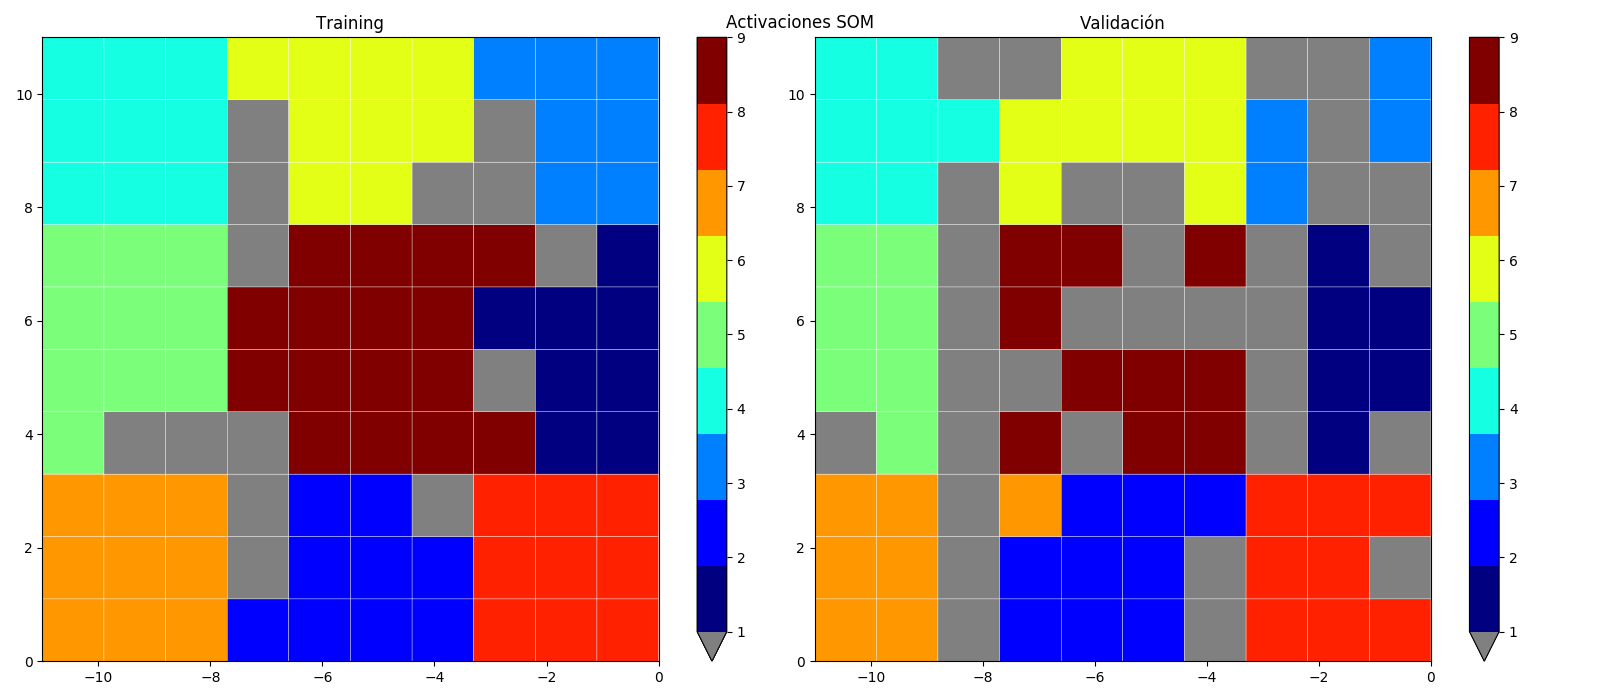
\includegraphics[width=160mm]{imagenes/som_10_10.png}
  \caption{Grilla de 10x10 sin preprocesamiento}
\end{figure}

\begin{figure}[H]
  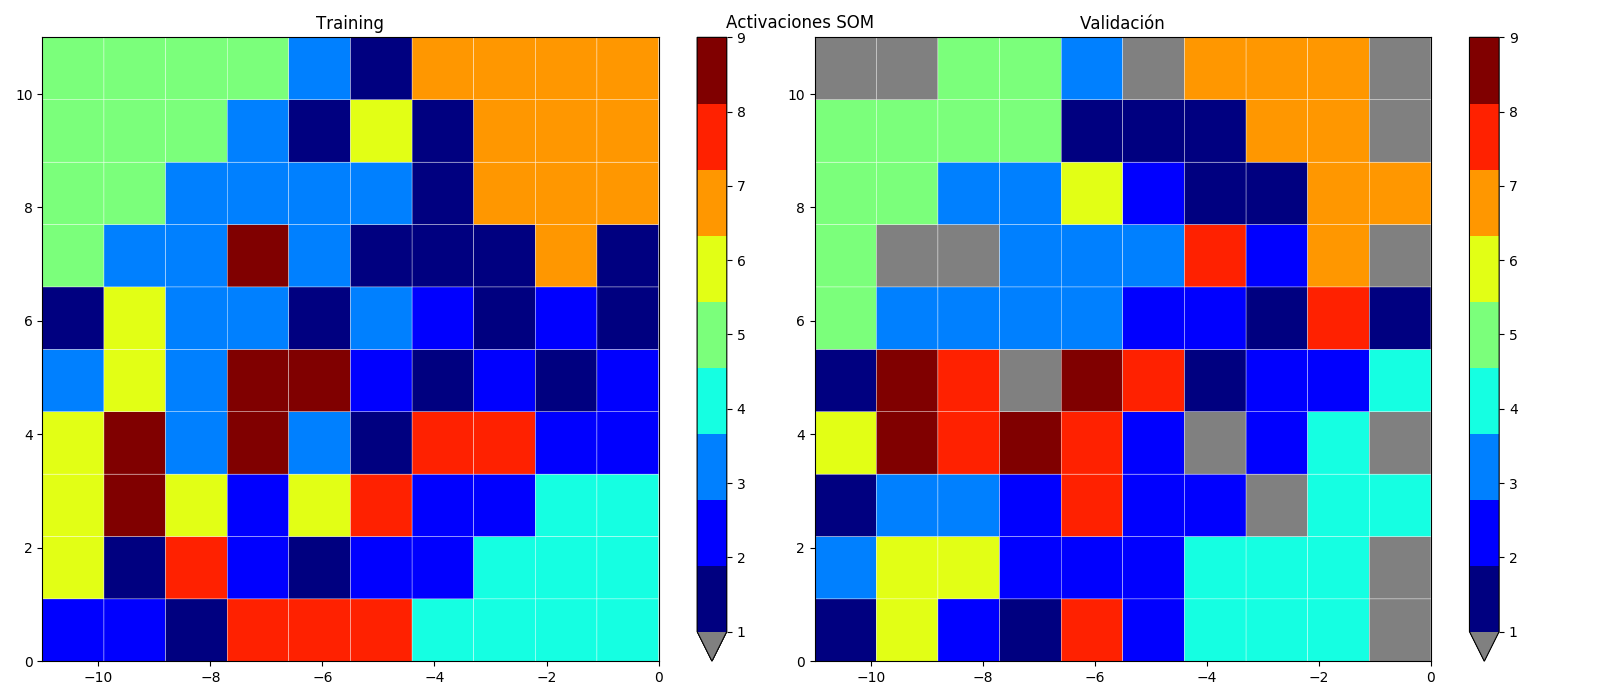
\includegraphics[width=160mm]{imagenes/som_10_10_3_preprocess.png}
  \caption{Grilla de 10x10 con preprocesamiento y 3 componentes principales}
\end{figure}

\begin{figure}[H]
  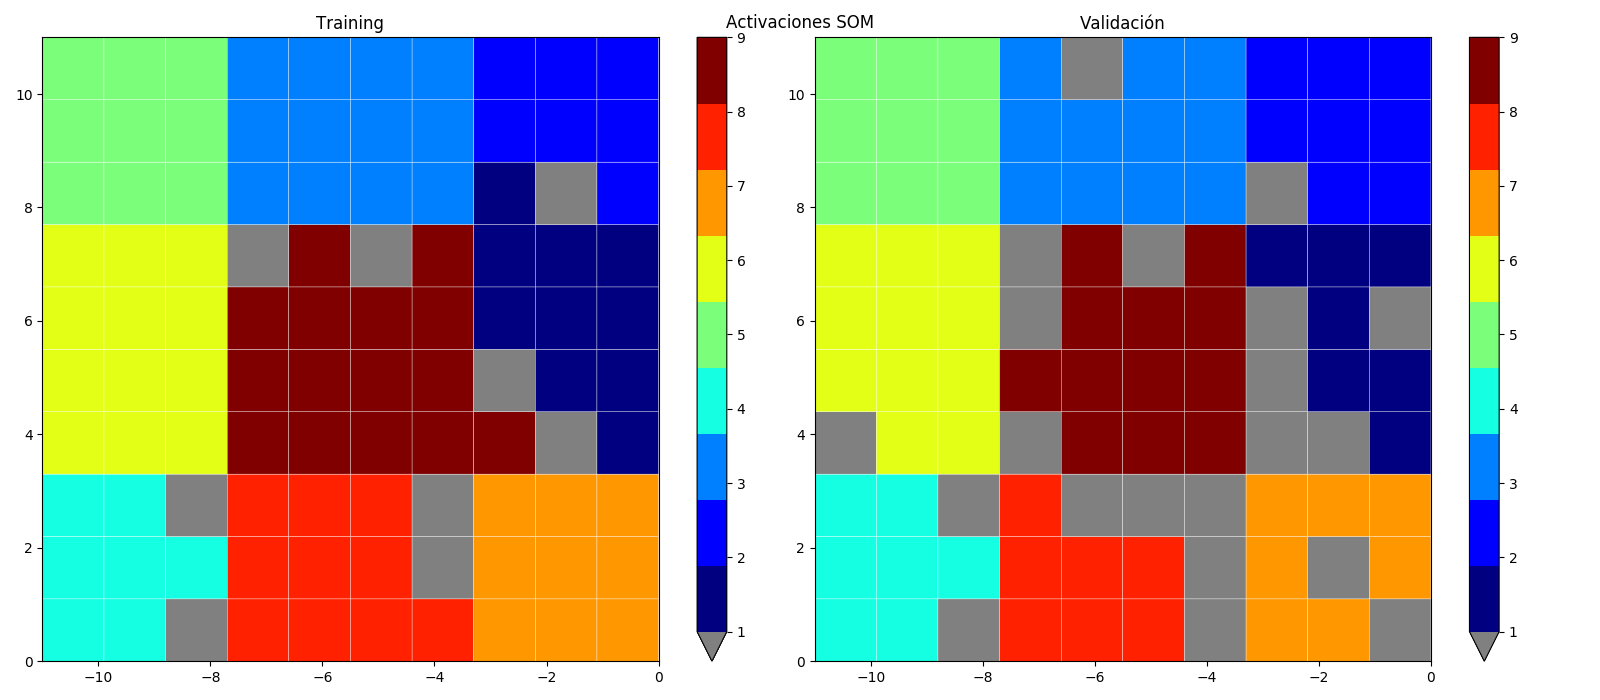
\includegraphics[width=160mm]{imagenes/som_10_10_9_preprocess.png}
  \caption{Grilla de 10x10 con preprocesamiento y 9 componentes principales}
\end{figure}

\begin{figure}[H]
  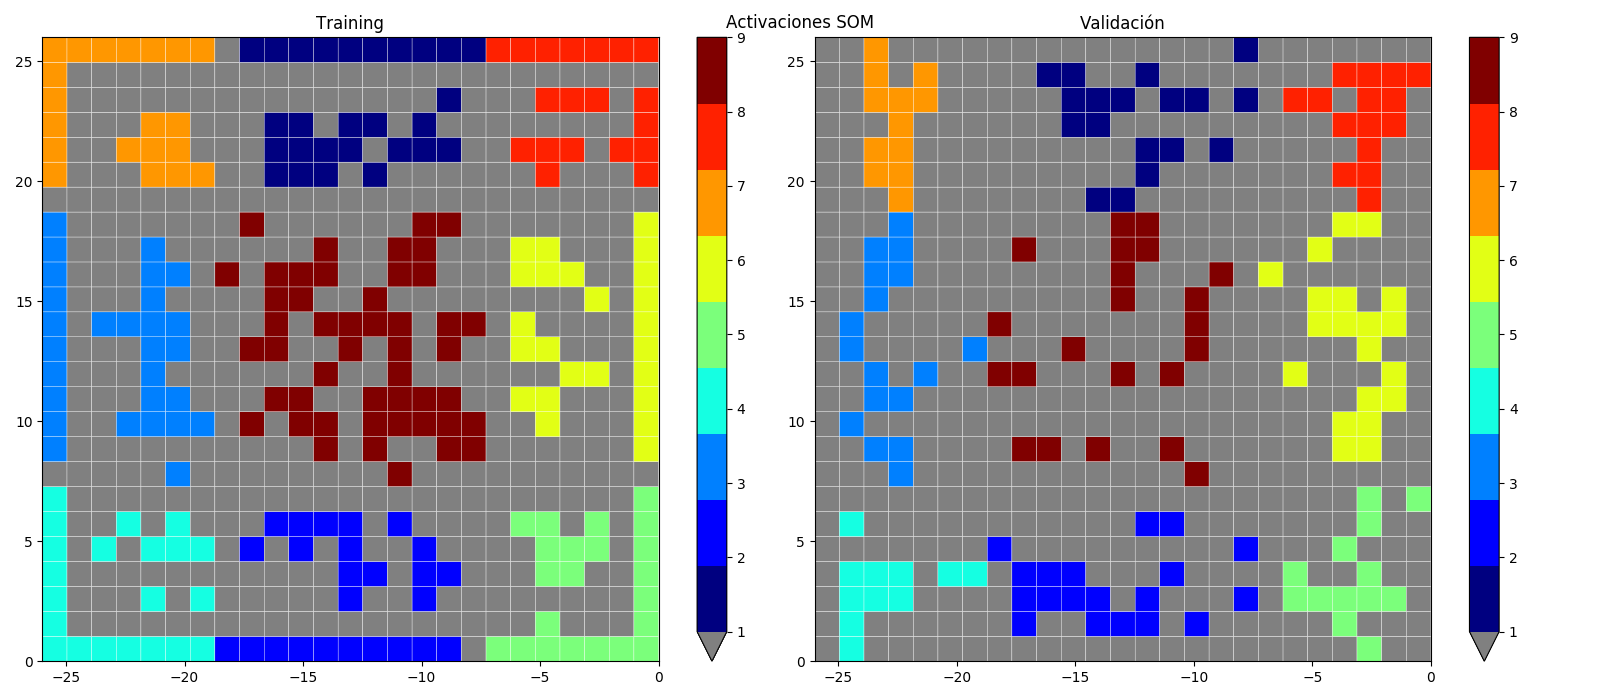
\includegraphics[width=160mm]{imagenes/som_25_25.png}
  \caption{Grilla de 25x25 sin preprocesamiento}
\end{figure}

\begin{figure}[H]
  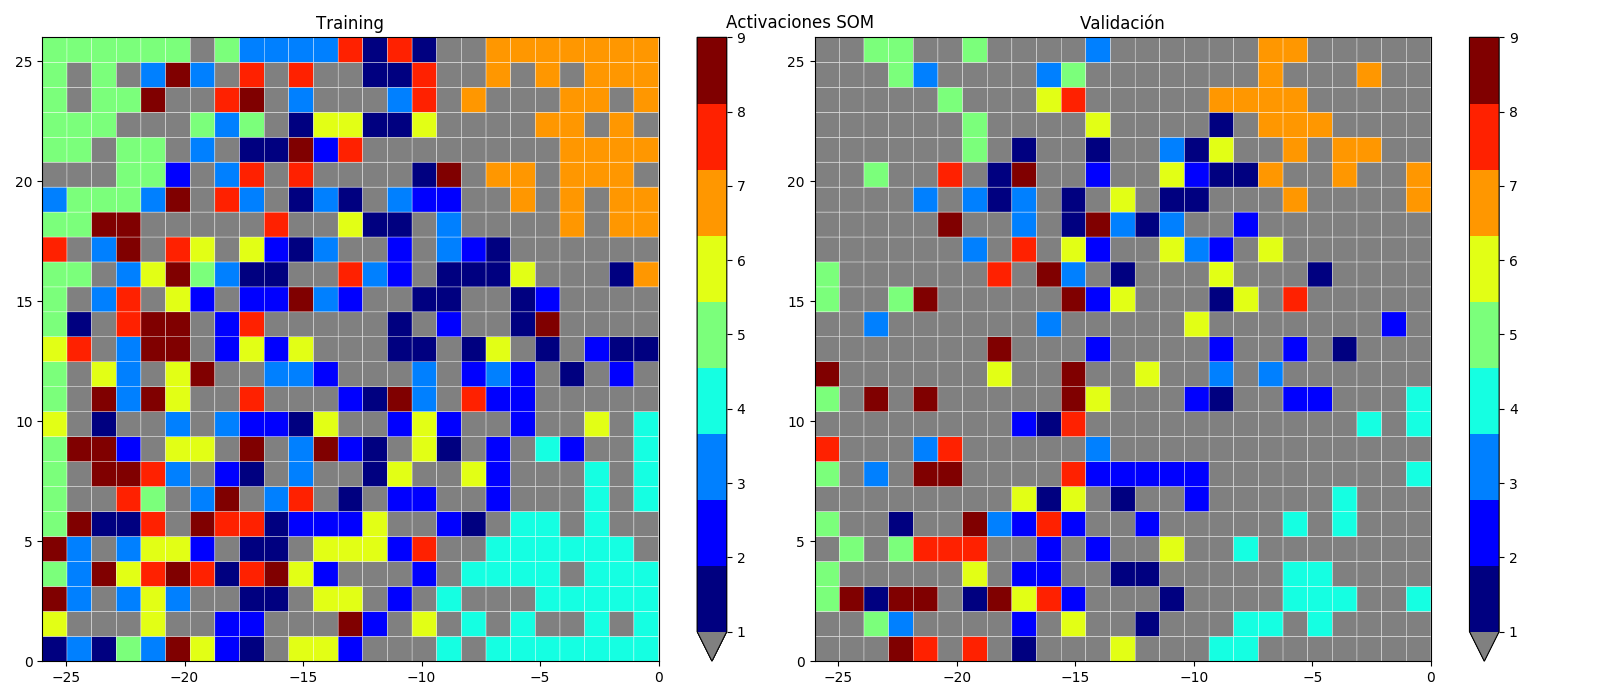
\includegraphics[width=160mm]{imagenes/som_25_25_3_preprocess.png}
  \caption{Grilla de 25x25 con preprocesamiento y 3 componentes principales}
\end{figure}

\begin{figure}[H]
  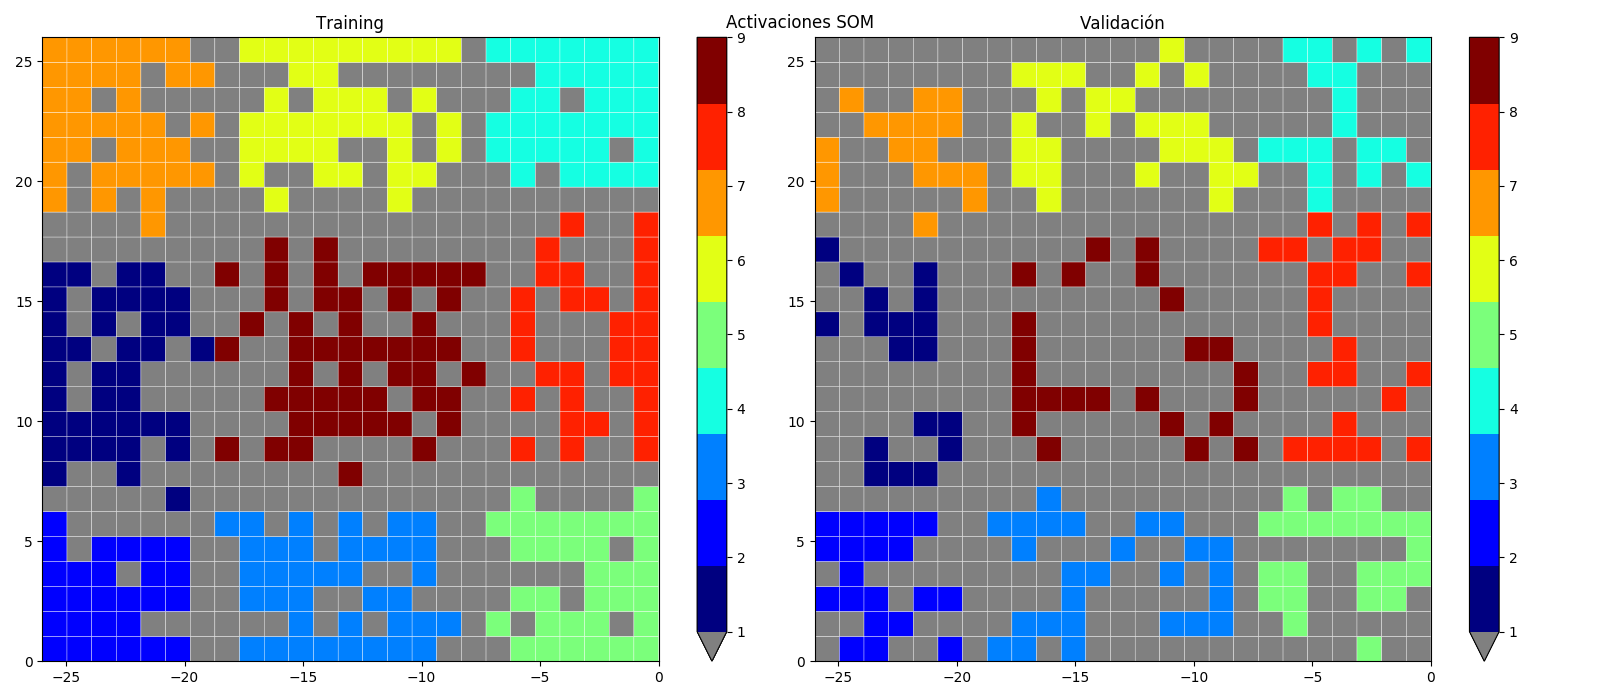
\includegraphics[width=160mm]{imagenes/som_25_25_9_preprocess.png}
  \caption{Grilla de 25x25 con preprocesamiento y 9 componentes principales}
\end{figure}

\subsection{Conclusión}
Una conclusion que se observo fue la diferencia en los tiempos de entrenamiento de la red con preprocesamiento
con respecto al entrenamiento sin preprocesado. Esto tiene sentido ya que se esta entrenando con una entrada de menor
dimensionalidad logrando que el computo realizado sea menor teniendo en cuenta aun el tiempo de  preprocesado.
 Con respecto a la calidad obtenida por cada experimento
se concluyo que la calidad de la red con preprocesamiento es superior a la red sin preprocesamiento, considerando calidad
la forma en la que la red agrupa instancias, es decir la forma de los clusters.

Con respecto a los datos de testeo se observo que el mapa generado presenta una mayor cantidad de neuronas en color gris,
esto quiere decir que hay mas neuronas que nunca se activan en el testing en comparacion con el entrenamiento.

Tambien se observo que al preprocesar tomando 3 componentes principales se pudieron distinguir 3 clusters del resto pero
sin poder diferenciarse entre si. El resto de los clusters se entremezclaron con facilidad sin lograr hacer una distincion.
Esto no sucedio cuando se tomaron 9 componentes principales, caso en el que se lograron visualizar los 9 clusters bien definidos.

Se observo que la red agrupa siempre en 9 clusters similares pero no siempre los mismos colores se mapean a las misma
distribucion espacial. Esto no ocurre con el cluster central que siempre le asigna la categoria 9 (color bordo).

\bibliographystyle{plain}
\bibliography{bibliografia}
\newpage
% \input{apendice}

\textbf{INVENTAR APRENDIZAJE QUE MINIMICE FALSOS NEGATIVOS}


\end{document}
